Since ancient times, mankind has constantly spent effort to create new or to improve existing tools.
Even now, after thousands and thousands of years we are doing the same.
We are making new tools that will make us more efficient or at least to do our tasks easier.
In software development there are so many tools available it is hard to choose which set should be used.
Next sections will give simple overview of most prominent tools for each section.


\section{Command line interfaces}\label{sec:command-line-interfaces}
Command line interfaces (CLI) are programs that use console/textual interface and allow you to interact with it.
Every operating system comes with one or more of these, Windows has Command Prompt (aka cmd.exe) and PowerShell,
Linux has sh and bash with many alternatives (commonly known as shell), and macOS has Terminal.app.
One issue that novice developers struggle is that when someone tells you to “open the terminal”,
they mean one for your system.

Before mentioned apps are the ones that allow you to execute some commands or run different programs.
There are also some CLI that is specifically built for one purpose.
One example would be Nest.js CLI which allows you to quickly create new projects,
update dependencies or start the Nest app.

\subsection{Command prompt}\label{subsec:command-prompt}
Command prompt comes preinstalled on Windows systems.
It supports batch scripts and usually the file is with .bat extension.

\noindent\begin{minipage}[t]{0.5\textwidth}%
    \centering{Pros}
    \begin{itemize}[leftmargin=*]
        \item Available on all Windows systems
        \item Allows executing programs in current directory without  \lstinline{.\}  prefix
    \end{itemize}
\end{minipage}%
\begin{minipage}[t]{0.5\textwidth}%
    \centering{Cons}
    \begin{itemize}[leftmargin=*]
        \item Batch scripting language is really outdated and hard to write more complex stuff
        \item No command history search
    \end{itemize}
\end{minipage}%

%! suppress = FigureNotReferenced
%! suppress = FigureNotReferenced
\begin{figure}[htbp]
    \centering
    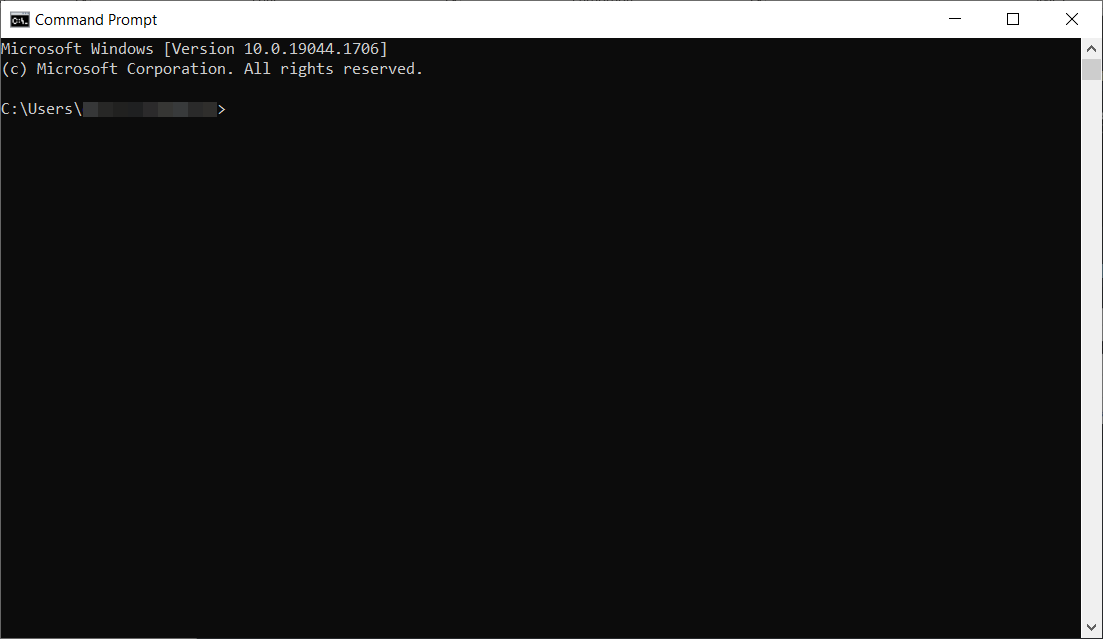
\includegraphics[width=0.6\textwidth]{images/command-prompt}
    \caption{Command Prompt\label{fig:Command Prompt}}
\end{figure}

Reference for available Command Prompt commands can be found at
\href{https://docs.microsoft.com/en-us/windows-server/administration/windows-commands/windows-commands}{Windows Commands}

\subsection{PowerShell}\label{subsec:powershell}
Another shell for Windows systems is called PowerShell, and it is available from Windows 7 or later operating systems.
Open source version PowerShell Core was released in 2016, and it is based on .Net Core which also made it cross-platform.
It has better integration with various functionalities available in Windows, so it is preferred choice to Command Prompt
when working with system administration.
For developer work it might be an overkill.


\noindent\begin{minipage}[t]{0.5\textwidth}%
    \centering{Pros}
    \begin{itemize}[leftmargin=*]
        \item Available on all Windows systems
        \item Better integration with Windows functionalities
        \item Has command history search (with F8 key)
    \end{itemize}
\end{minipage}%
\begin{minipage}[t]{0.5\textwidth}%
    \centering{Cons}
    \begin{itemize}[leftmargin=*]
        \item  Does not allow executing programs in
              current directory without  \lstinline{.\} prefix
    \end{itemize}
\end{minipage}%

%! suppress = FigureNotReferenced
\begin{figure}[htbp]
    \centering
    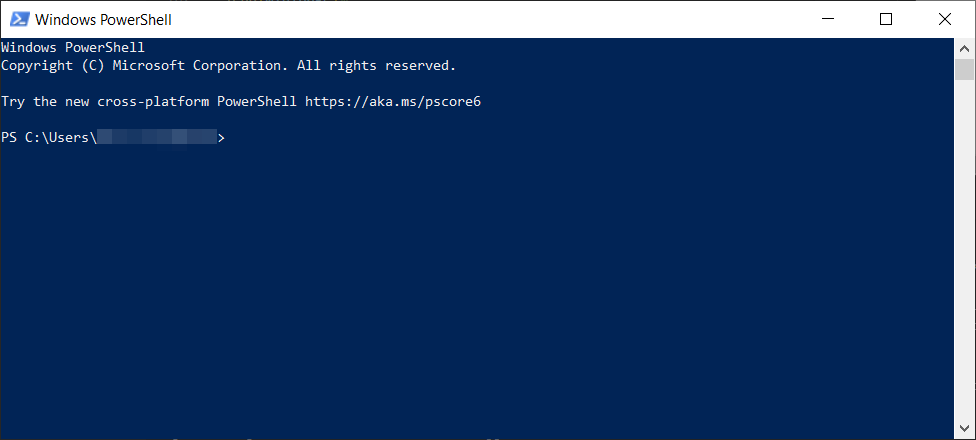
\includegraphics[width=0.6\textwidth]{images/powershell}
    \caption{PowerShell\label{fig:PowerShell}}
\end{figure}

\subsection{Linux/Mac terminals/shells}\label{subsec:linux/mac-terminals/shells}

Linux and Mac have much bigger choice of terminals.
Terminal refers to a program that allows you to run programs which are known as shells.
Shells come in lots of varieties sh, bash, ksh, csh, zsh\dots.
Linux has many command line programs that allow you to manipulate output of commands and offers a lot for power users.


\section{Package managers}\label{sec:package-managers}

Package managers can be used to install additional software on your PC. They usually automate process of
downloading, installing and configuring software.
Later it also helps with keeping the installed software up to date or with removal.

\begin{itemize}[leftmargin=*]
    \item Windows: Chocolatey is the most prominent package manager.
    It can be downloaded from \href{https://chocolatey.org/}{https://chocolatey.org/}.
    Searching for packages is done with \mintinline{bat}{choco search postgresql}
    and installation with \mintinline{bat}{choco install postgresql} will install Postgres.
    \item Windows: Winget is the alternative package manager created by Microsoft.
    It can be downloaded from \href{https://chocolatey.org/}{https://chocolatey.org/}.
    Searching for packages is done with \mintinline{bat}{winget search postgres}
    and installation with \mintinline{bat}{winget install postgresql} will install Postgres.
    \item Mac OS X: Homebrew is a package manager written in Ruby.
          It can be downloaded from \href{https://brew.sh}{https://brew.sh}.
          Command \mintinline{bat}{brew search postgres}
          is used to search for package while \mintinline{bat}{brew install postgresql} to install a package.
    \item Linux has many package managers and preferred way is to use package manager
          that comes with operating system.
\end{itemize}